% ***************************************************************************************************
% A Classic Thesis Style
% An Homage to The Elements of Typographic Style
%
% Copyright (C) 2017 André Miede and Ivo Pletikosić
%
% License:
% This program is free software; you can redistribute it and/or modify
% it under the terms of the GNU General Public License as published by
% the Free Software Foundation; either version 2 of the License, or
% (at your option) any later version.
%
% This program is distributed in the hope that it will be useful,
% but WITHOUT ANY WARRANTY; without even the implied warranty of
% MERCHANTABILITY or FITNESS FOR A PARTICULAR PURPOSE.  See the
% GNU General Public License for more details.
%
% You should have received a copy of the GNU General Public License
% along with this program; see the file COPYING.  If not, write to
% the Free Software Foundation, Inc., 59 Temple Place - Suite 330,
% Boston, MA 02111-1307, USA.
%
% PLEASE SEE ALSO THE AUTHORS' NOTE REGARDING THIS LICENSE
% IN THE DOCUMENTATION (ClassicThesis.pdf --> Chapter 1 / Chapter01.tex)
% **************************************************************************************************

\RequirePackage{silence} % :-\
    \WarningFilter{scrreprt}{Usage of package `titlesec'}
    %\WarningFilter{scrreprt}{Activating an ugly workaround}
    \WarningFilter{titlesec}{Non standard sectioning command detected}

\documentclass[twoside,openright,titlepage,numbers=noenddot,headinclude,%1headlines,% letterpaper a4paper
               footinclude=true,cleardoublepage=empty,abstractoff, % <--- obsolete, remove (todo)
               BCOR=5mm,paper=a4,fontsize=11pt,%11pt,a4paper,%
               ngerman,american,%
               ]{scrreprt}


%********************************************************************
% Note: Make all your adjustments in here
%*******************************************************
% ****************************************************************************************************
% classicthesis-config.tex
% formerly known as loadpackages.sty, classicthesis-ldpkg.sty, and classicthesis-preamble.sty
% Use it at the beginning of your ClassicThesis.tex, or as a LaTeX Preamble
% in your ClassicThesis.{tex,lyx} with \input{classicthesis-config}
% ****************************************************************************************************
% If you like the classicthesis, then I would appreciate a postcard.
% My address can be found in the file ClassicThesis.pdf. A collection
% of the postcards I received so far is available online at
% http://postcards.miede.de
% ****************************************************************************************************


% ****************************************************************************************************
% 0. Set the encoding of your files. UTF-8 is the only sensible encoding nowadays. If you can't read
% äöüßáéçèê∂åëæƒÏ€ then change the encoding setting in your editor, not the line below. If your editor
% does not support utf8 use another editor!
% ****************************************************************************************************
\PassOptionsToPackage{utf8}{inputenc}
  \usepackage{inputenc}

% ****************************************************************************************************
% 1. Configure classicthesis for your needs here, e.g., remove "drafting" below
% in order to deactivate the time-stamp on the pages
% (see ClassicThesis.pdf for more information):
% ****************************************************************************************************
\PassOptionsToPackage{
  drafting=true,    % print version information on the bottom of the pages
  tocaligned=false, % the left column of the toc will be aligned (no indentation)
  dottedtoc=true,   % page numbers in ToC flushed right
  parts=true,       % use part division
  eulerchapternumbers=true, % use AMS Euler for chapter font (otherwise Palatino)
  linedheaders=false,       % chaper headers will have line above and beneath
  floatperchapter=true,     % numbering per chapter for all floats (i.e., Figure 1.1)
  listings=true,    % load listings package and setup LoL
  subfig=true,      % setup for preloaded subfig package
  eulermath=false,  % use awesome Euler fonts for mathematical formulae (only with pdfLaTeX)
  beramono=true,    % toggle a nice monospaced font (w/ bold)
  minionpro=false   % setup for minion pro font; use minion pro small caps as well (only with pdfLaTeX)
}{researchbook}


% ****************************************************************************************************
% 2. Personal data and user ad-hoc commands
% ****************************************************************************************************
\newcommand{\myTitle}{Summary of My Research\xspace}
\newcommand{\mySubtitle}{From The Academia to The Industry: The Precious Journey\xspace}
\newcommand{\myDegree}{Ph.D.\xspace}
\newcommand{\myName}{Siyang Xie\xspace}
\newcommand{\myProf}{Yanfeng Ouyang\xspace}
\newcommand{\myOtherProf}{Hai Jiang\xspace}
\newcommand{\mySupervisor}{Put name here\xspace}
\newcommand{\myFaculty}{Put data here\xspace}
\newcommand{\myDepartment}{Civil and Environmental Engineering\xspace}
\newcommand{\myGradUniv}{University of Illinois at Urbana-Champaign\xspace}
\newcommand{\myUgradUniv}{Tsinghua University\xspace}
\newcommand{\myLocation}{Saarbrücken\xspace}
\newcommand{\myTime}{February 2018\xspace}
\newcommand{\myVersion}{version 1.0}

% ********************************************************************
% Setup, finetuning, and useful commands
% ********************************************************************
\newcounter{dummy} % necessary for correct hyperlinks (to index, bib, etc.)
\newlength{\abcd} % for ab..z string length calculation
\providecommand{\mLyX}{L\kern-.1667em\lower.25em\hbox{Y}\kern-.125emX\@}
\newcommand{\ie}{i.\,e.}
\newcommand{\Ie}{I.\,e.}
\newcommand{\eg}{e.\,g.}
\newcommand{\Eg}{E.\,g.}
% ****************************************************************************************************


% ****************************************************************************************************
% 3. Loading some handy packages
% ****************************************************************************************************
% ********************************************************************
% Packages with options that might require adjustments
% ********************************************************************
%\PassOptionsToPackage{ngerman,american}{babel}   % change this to your language(s), main language last
% Spanish languages need extra options in order to work with this template
%\PassOptionsToPackage{spanish,es-lcroman}{babel}
\usepackage{babel}

\usepackage{csquotes}
\PassOptionsToPackage{%
  %backend=biber,bibencoding=utf8, %instead of bibtex
  backend=bibtex8,
  bibencoding=ascii,%
  language=auto,%
  style=numeric-comp,%
  %style=authoryear-comp, % Author 1999, 2010
  %bibstyle=authoryear,dashed=false, % dashed: substitute rep. author with ---
  sorting=nyt, % name, year, title
  maxbibnames=10, % default: 3, et al.
  %backref=true,%
  natbib=true % natbib compatibility mode (\citep and \citet still work)
}{biblatex}
\usepackage{biblatex}

% \PassOptionsToPackage{fleqn}{amsmath}  % math environments Position equations at a fixed indent from the left margin rather than centered in the text column.

\usepackage{amsmath}

% ********************************************************************
% General useful packages
% ********************************************************************
\PassOptionsToPackage{T1}{fontenc} % T2A for cyrillics
\usepackage{fontenc}
\usepackage{textcomp} % fix warning with missing font shapes
\usepackage{scrhack} % fix warnings when using KOMA with listings package
\usepackage{xspace} % to get the spacing after macros right
\usepackage{mparhack} % get marginpar right
%\usepackage{fixltx2e} % fixes some LaTeX stuff --> since 2015 in the LaTeX kernel (see below)
% \usepackage[latest]{latexrelease} % emulate newer kernel version if older is detected
\PassOptionsToPackage{printonlyused,smaller}{acronym}
  \usepackage{acronym} % nice macros for handling all acronyms in the thesis
  %\renewcommand{\bflabel}[1]{{#1}\hfill} % fix the list of acronyms --> no longer working
  %\renewcommand*{\acsfont}[1]{\textsc{#1}}
  %\renewcommand*{\aclabelfont}[1]{\acsfont{#1}}
  %\def\bflabel#1{{#1\hfill}}
  \def\bflabel#1{{\acsfont{#1}\hfill}}
  \def\aclabelfont#1{\acsfont{#1}}
% ****************************************************************************************************
%\usepackage{pgfplots} % External TikZ/PGF support (thanks to Andreas Nautsch)
%\usetikzlibrary{external}
%\tikzexternalize[mode=list and make, prefix=ext-tikz/]
% ****************************************************************************************************


% ****************************************************************************************************
% 4. Setup floats: tables, (sub)figures, and captions
% ****************************************************************************************************
\usepackage{tabularx} % better tables
  % \setlength{\extrarowheight}{3pt} % increase table row height
\newcommand{\tableheadline}[1]{\multicolumn{1}{c}{\spacedlowsmallcaps{#1}}}
\newcommand{\myfloatalign}{\centering} % to be used with each float for alignment
\usepackage{caption}
% Thanks to cgnieder and Claus Lahiri
% http://tex.stackexchange.com/questions/69349/spacedlowsmallcaps-in-caption-label
% [REMOVED DUE TO OTHER PROBLEMS, SEE ISSUE #82]
%\DeclareCaptionLabelFormat{smallcaps}{\bothIfFirst{#1}{~}\MakeTextLowercase{\textsc{#2}}}
%\captionsetup{font=small,labelformat=smallcaps} % format=hang,
\captionsetup{font=large} % format=hang,
\usepackage{algorithmthesis}
\usepackage{subfigure}
\usepackage{graphicx,graphics}
\usepackage{enumerate}
\usepackage{multirow}
\usepackage{array,bigstrut}
\usepackage{booktabs,makecell}
\usepackage{amsthm,amssymb,bm}
\usepackage{blindtext}
\usepackage{url}
\usepackage[hidelinks]{hyperref}
\hypersetup{breaklinks=true}
\urlstyle{same}

\makeatletter
\DeclareOldFontCommand{\rm}{\normalfont\rmfamily}{\mathrm}
\DeclareOldFontCommand{\sf}{\normalfont\sffamily}{\mathsf}
\DeclareOldFontCommand{\tt}{\normalfont\ttfamily}{\mathtt}
\DeclareOldFontCommand{\bf}{\normalfont\bfseries}{\mathbf}
\DeclareOldFontCommand{\it}{\normalfont\itshape}{\mathit}
\DeclareOldFontCommand{\sl}{\normalfont\slshape}{\@nomath\sl}
\DeclareOldFontCommand{\sc}{\normalfont\scshape}{\@nomath\sc}
\makeatother


% ****************************************************************************************************


% ****************************************************************************************************
% 5. Setup code listings
% ****************************************************************************************************
\usepackage{listings}
%\lstset{emph={trueIndex,root},emphstyle=\color{BlueViolet}}%\underbar} % for special keywords
\lstset{language=[LaTeX]Tex,%C++,
  morekeywords={PassOptionsToPackage,selectlanguage},
  keywordstyle=\color{RoyalBlue},%\bfseries,
  basicstyle=\small\ttfamily,
  %identifierstyle=\color{NavyBlue},
  commentstyle=\color{Green}\ttfamily,
  stringstyle=\rmfamily,
  numbers=none,%left,%
  numberstyle=\scriptsize,%\tiny
  stepnumber=5,
  numbersep=8pt,
  showstringspaces=false,
  breaklines=true,
  %frameround=ftff,
  %frame=single,
  belowcaptionskip=.75\baselineskip
  %frame=L
}
% ****************************************************************************************************


% ****************************************************************************************************
% 6. PDFLaTeX, hyperreferences, and citation backreferences
% ****************************************************************************************************
% ********************************************************************
% Using PDFLaTeX
% ********************************************************************
\PassOptionsToPackage{hyperfootnotes=false,pdfpagelabels}{hyperref}
  \usepackage{hyperref}  % backref linktocpage pagebackref
%\ifpdf
%\pdfcompresslevel=9
%\pdfadjustspacing=1
%\fi
%\PassOptionsToPackage{pdftex}{graphicx} %%%IVO: driver will be chosen automatically
  \usepackage{graphicx}


% ********************************************************************
% Hyperreferences
% ********************************************************************
\hypersetup{%
  %draft, % hyperref's draft mode, for printing see below
  colorlinks=true, linktocpage=true, pdfstartpage=3, pdfstartview=FitV,%
  % uncomment the following line if you want to have black links (e.g., for printing)
  %colorlinks=false, linktocpage=false, pdfstartpage=3, pdfstartview=FitV, pdfborder={0 0 0},%
  breaklinks=true, pdfpagemode=UseNone, pageanchor=true, pdfpagemode=UseOutlines,%
  plainpages=false, bookmarksnumbered, bookmarksopen=true, bookmarksopenlevel=1,%
  hypertexnames=true, pdfhighlight=/O,%nesting=true,%frenchlinks,%
  urlcolor=webbrown, linkcolor=RoyalBlue, citecolor=webgreen, %pagecolor=RoyalBlue,%
  %urlcolor=Black, linkcolor=Black, citecolor=Black, %pagecolor=Black,%
  pdftitle={\myTitle},%
  pdfauthor={\textcopyright\ \myName, \myGradUniv, \myUgradUniv},%
  pdfsubject={},%
  pdfkeywords={},%
  pdfcreator={pdfLaTeX},%
  %pdfproducer={LaTeX with hyperref and researchbook}%
}

% ********************************************************************
% Setup autoreferences
% ********************************************************************
% There are some issues regarding autorefnames
% http://www.ureader.de/msg/136221647.aspx
% http://www.tex.ac.uk/cgi-bin/texfaq2html?label=latexwords
% you have to redefine the makros for the
% language you use, e.g., american, ngerman
% (as chosen when loading babel/AtBeginDocument)
% ********************************************************************
\makeatletter
% \theoremstyle{plain}
\newtheorem{defn}{Definition}
\newtheorem{prop}{Proposition}
\newtheorem{theorem}{Theorem}
\newtheorem{lemma}{Lemma}
\newtheorem{cor}{Corollary}
\newtheorem{rem}{Remark}

\@ifpackageloaded{babel}%
  {%
    \addto\extrasamerican{%
      \renewcommand*{\figureautorefname}{Figure}%
      \renewcommand*{\tableautorefname}{Table}%
      \renewcommand*{\partautorefname}{Part}%
      \renewcommand*{\chapterautorefname}{Chapter}%
      \renewcommand*{\sectionautorefname}{Section}%
      \renewcommand*{\subsectionautorefname}{Section}%
      \renewcommand*{\subsubsectionautorefname}{Section}%
      \providecommand*\defnautorefname{Definition}
      \providecommand*\propautorefname{Proposition}
      \providecommand*\thmautorefname{Theorem}
      \providecommand*\lemautorefname{Lemma}
      \providecommand*\corautorefname{Corollary}
      \providecommand*\remautorefname{Remark}
    }%
    \addto\extrasngerman{%
      \renewcommand*{\paragraphautorefname}{Absatz}%
      \renewcommand*{\subparagraphautorefname}{Unterabsatz}%
      \renewcommand*{\footnoteautorefname}{Fu\"snote}%
      \renewcommand*{\FancyVerbLineautorefname}{Zeile}%
      \renewcommand*{\theoremautorefname}{Theorem}%
      \renewcommand*{\appendixautorefname}{Anhang}%
      \renewcommand*{\equationautorefname}{Gleichung}%
      \renewcommand*{\itemautorefname}{Punkt}%
    }%
      % Fix to getting autorefs for subfigures right (thanks to Belinda Vogt for changing the definition)
      \providecommand{\subfigureautorefname}{\figureautorefname}%
    }{\relax}
\makeatother


\usepackage{calc}
\usepackage{mdwlist}
\newenvironment{notation}[1][1.2cm]{
  \noindent\begin{list}{}%
    {\vskip-30bp
     \renewcommand\makelabel[1]{##1\hfil}
     \setlength{\labelwidth}{#1}
     \setlength{\labelsep}{0.8cm}
     \setlength{\itemindent}{0cm}
     \setlength{\leftmargin}{\labelwidth+\labelsep}
     \setlength{\rightmargin}{0cm}
     \setlength{\parsep}{0cm}
     \setlength{\itemsep}{0cm}
    \setlength{\listparindent}{0cm}
    \setlength{\topsep}{0pt}
  }}{\end{list}}


% ****************************************************************************************************
% 7. Last calls before the bar closes
% ****************************************************************************************************
% ********************************************************************
% Development Stuff
% ********************************************************************
\listfiles
%\PassOptionsToPackage{l2tabu,orthodox,abort}{nag}
%  \usepackage{nag}
%\PassOptionsToPackage{warning, all}{onlyamsmath}
%  \usepackage{onlyamsmath}

% ********************************************************************
% Last, but not least...
% ********************************************************************
\usepackage{researchbook}
% ****************************************************************************************************


% ****************************************************************************************************
% 8. Further adjustments (experimental)
% ****************************************************************************************************
% ********************************************************************
% Changing the text area
% ********************************************************************
%\areaset[current]{312pt}{761pt} % 686 (factor 2.2) + 33 head + 42 head \the\footskip
%\setlength{\marginparwidth}{7em}%
%\setlength{\marginparsep}{2em}%

% ********************************************************************
% Using different fonts
% ********************************************************************
%\usepackage[oldstylenums]{kpfonts} % oldstyle notextcomp
%\usepackage[osf]{libertine}
%\usepackage[light,condensed,math]{iwona}
%\renewcommand{\sfdefault}{iwona}
%\usepackage{lmodern} % <-- no osf support :-(
%\usepackage{cfr-lm} %
%\usepackage[urw-garamond]{mathdesign} <-- no osf support :-(
%\usepackage[default,osfigures]{opensans} % scale=0.95
%\usepackage[sfdefault]{FiraSans}
% ********************************************************************
% \usepackage[largesc,osf]{newpxtext}
% Used to fix these:
% https://bitbucket.org/amiede/classicthesis/issues/139/italics-in-pallatino-capitals-chapter
% https://bitbucket.org/amiede/classicthesis/issues/45/problema-testatine-su-classicthesis-style
% ********************************************************************
%\linespread{1.05} % a bit more for Palatino
% ****************************************************************************************************



%********************************************************************
% Bibliographies
%*******************************************************
\addbibresource{thesisrefs.bib}
\addbibresource[label=ownpubs]{Siyang_Publications.bib}
\addbibresource[label=ownmanus]{Siyang_Manuscripts.bib}
%\renewcommand*{\bibname}{new name}
%\setbibpreamble{}


%********************************************************************
% Hyphenation
%********************************************************************
%\hyphenation{put special hyphenation here}



\begin{document}


%\frenchspacing
\raggedbottom
\selectlanguage{american} % american ngerman
\pagenumbering{roman}
\pagestyle{plain}



%********************************************************************
% Frontmatter
%********************************************************************
%*******************************************************
% Titlepage
%*******************************************************
\begin{titlepage}
    % if you want the titlepage to be centered, uncomment and fine-tune the line below (KOMA classes environment)
    \begin{addmargin}[-1cm]{-3cm}
    \begin{center}
        \large

        \hfill

        \vfill

        \begingroup
            \color{Maroon}\spacedallcaps{\LARGE \myTitle} \\ \bigskip
        \endgroup
        \vskip 2em
        \spacedallcaps{\myName}

        \vfill

        % \includegraphics[width=6cm]{gfx/TFZsuperellipse_bw} \\ \medskip

        \mySubtitle \\ \medskip
        %\myDegree \\
        %\myDepartment \\
        %\myFaculty \\
        %\myUni \\ \bigskip

        \myTime\ -- \myVersion

        \vfill

    \end{center}
  \end{addmargin}
\end{titlepage}

\thispagestyle{empty}

\hfill

\vfill

\noindent\myName: \textit{\myTitle,} \mySubtitle, %\myDegree,
\textcopyright\ \myTime

\bigskip

\noindent\spacedlowsmallcaps{Supervisors}: \\
\myProf, \myGradUniv \\
\myOtherProf, \myUgradUniv
% \mySupervisor

% \medskip

% \noindent\spacedlowsmallcaps{Location}: \\
% \myLocation

\medskip

\noindent\spacedlowsmallcaps{Time Frame}: \\
October 2010 -- \myTime
\cleardoublepage
%*******************************************************
% Abstract
%*******************************************************
%\renewcommand{\abstractname}{Abstract}
\pdfbookmark[1]{Abstract}{Abstract}
\begingroup
\let\clearpage\relax
\let\cleardoublepage\relax
\let\cleardoublepage\relax

\chapter*{Abstract}
Summary of the research I have done in the past almost ten years. More information can be found here:
% \begin{center}
\url{https://www.siyangxie.com}
% \end{center}

\vfill

% \begin{otherlanguage}{ngerman}
% \pdfbookmark[1]{Zusammenfassung}{Zusammenfassung}
% \chapter*{Zusammenfassung}
% Kurze Zusammenfassung des Inhaltes in deutscher Sprache\dots
% \end{otherlanguage}

\endgroup

\vfill
\cleardoublepage
%*******************************************************
% Acknowledgments
%*******************************************************
\pdfbookmark[1]{Acknowledgments}{acknowledgments}

\begin{flushright}{\slshape
    There is no mistake in a tango, \\ \medskip
    not like life.} \\ \medskip
    --- Al Pacino as Lieutenant Colonel Frank Slade, Scent of a Woman
\end{flushright}



\bigskip

\begingroup
\let\clearpage\relax
\let\cleardoublepage\relax
\let\cleardoublepage\relax
\chapter*{Acknowledgments}

\noindent Many thanks to my advisors, Professor Yanfeng Ouyang, and Professor Hai Jiang.

\noindent Special thanks to my family and close friends for accompanying me along the way.


% \bigskip

% \noindent\emph{Regarding \mLyX}: The \mLyX\ port was intially done by


\endgroup



\cleardoublepage
%*******************************************************
% Publications
%*******************************************************
\pdfbookmark[1]{Publications}{publications}
\chapter*{Publications}\graffito{This is the current list of my publications}
Most of the contents in the book have appeared previously in the following publications:

%\noindent Put your publications from the thesis here. The packages \texttt{multibib} or \texttt{bibtopic} etc. can be used to handle multiple different bibliographies in your document.

\vskip 1em
\noindent \textbf{Paper Published In Journals}
\begin{refsection}[ownpubs]
    \small
    \nocite{*} % is local to to the enclosing refsection
    \printbibliography[heading=none]
\end{refsection}


\vskip 1em
\noindent \textbf{Manuscripts Submitted or In Preparation}
\begin{refsection}[ownmanus]
    \small
    \nocite{*} % is local to to the enclosing refsection
    \printbibliography[heading=none]
\end{refsection}

% \emph{Attention}: This requires a separate run of \texttt{bibtex} for your \texttt{refsection}, \eg, \texttt{ClassicThesis1-blx} for this file. You might also use \texttt{biber} as the backend for \texttt{biblatex}. See also \url{http://tex.stackexchange.com/questions/128196/problem-with-refsection}.
\cleardoublepage
%*******************************************************
% Table of Contents
%*******************************************************
\pagestyle{scrheadings}
%\phantomsection
\refstepcounter{dummy}
\pdfbookmark[1]{\contentsname}{tableofcontents}
\setcounter{tocdepth}{2} % <-- 2 includes up to subsections in the ToC
\setcounter{secnumdepth}{3} % <-- 3 numbers up to subsubsections
\manualmark
\markboth{\spacedlowsmallcaps{\contentsname}}{\spacedlowsmallcaps{\contentsname}}
\tableofcontents
\automark[section]{chapter}
\renewcommand{\chaptermark}[1]{\markboth{\spacedlowsmallcaps{#1}}{\spacedlowsmallcaps{#1}}}
\renewcommand{\sectionmark}[1]{\markright{\thesection\enspace\spacedlowsmallcaps{#1}}}
%*******************************************************
% List of Figures and of the Tables
%*******************************************************
\clearpage
% \pagestyle{empty} % Uncomment this line if your lists should not have any headlines with section name and page number
\begingroup
    \let\clearpage\relax
    \let\cleardoublepage\relax
    %*******************************************************
    % List of Figures
    %*******************************************************
    %\phantomsection
    \refstepcounter{dummy}
    %\addcontentsline{toc}{chapter}{\listfigurename}
    \pdfbookmark[1]{\listfigurename}{lof}
    \listoffigures

    \vspace{8ex}
    % \newpage

    %*******************************************************
    % List of Tables
    %*******************************************************
    \let\clearpage\relax
    \let\cleardoublepage\relax
    %\phantomsection
    \refstepcounter{dummy}
    %\addcontentsline{toc}{chapter}{\listtablename}
    \pdfbookmark[1]{\listtablename}{lot}
    \listoftables

    \vspace{8ex}
    % \newpage

    %*******************************************************
    % List of Listings
    %*******************************************************
    \let\clearpage\relax
    \let\cleardoublepage\relax
    %\phantomsection
    \refstepcounter{dummy}
    %\addcontentsline{toc}{chapter}{\lstlistlistingname}
    \pdfbookmark[1]{\lstlistlistingname}{lol}
    \lstlistoflistings

    \vspace{8ex}

    %*******************************************************
    % Acronyms
    %*******************************************************
    \let\clearpage\relax
    \let\cleardoublepage\relax
    %\phantomsection
    \refstepcounter{dummy}
    \pdfbookmark[1]{Acronyms}{acronyms}
    \markboth{\spacedlowsmallcaps{Acronyms}}{\spacedlowsmallcaps{Acronyms}}
    \chapter*{Acronyms}
    \begin{acronym}[UMLX]
        \acro{DRY}{Don't Repeat Yourself}
        \acro{API}{Application Programming Interface}
        \acro{UML}{Unified Modeling Language}
    \end{acronym}

\endgroup
\cleardoublepage



%********************************************************************
% Mainmatter
%********************************************************************

\pagestyle{scrheadings}
\pagenumbering{arabic}
%\setcounter{page}{90}
\cleardoublepage


\part{PhD Dissertation: RELIABLE FACILITY LOCATION}\label{part:dissertation}
% !TEX root = ../ResearchBook.tex

\chapter{Introduction}\label{chap:introduction}



\section{Motivation}\label{sec:intro-motivation}

Facility location decisions lie at the center of planning many infrastructure systems. In many practice, public agencies (e.g., governments) and private companies (e.g., retailers) both need to locate their facilities to serve spatially distributed demands/customers. For example, governments locate various public facilities, such as hospitals, schools, fire stations, to provide public services; retail companies determine the locations of their facilities including warehouses, assembly plants, stores, etc, to sell goods and provide business. The design of all such facility systems generally involves considerations of fixed investment of facility construction and transportation cost of serving demands, so as to maximize the operational efficiency and service profit of the system \citep{Daskin-2005}.


\section{Outline}\label{sec:intro-outline}

This dissertation is organized as follows. \autoref{chap:sensor} applies the reliable facility location modeling framework to sensor deployment context, in which sensors work in combinations to provide combinatorial service. The ideas of supporting stations are adopted with adjustment to represent the combinations of sensors. A mixed-integer mathematical model is formulated to determine the optimal sensor locations, the sensor combination plans, and the backup assignment decisions. Several approximation subroutines are carefully designed inside a Lagrangian relaxation framework to solve the model.  


% !TEX root = ../ResearchBook.tex

\chapter{RFL with Facility Combinations: Reliable Sensor Deployment for Positioning/Surveillance via Trilateration}\label{chap:sensor}
\chaptermark{RFL with Facility Combinations: Sensor}

In this chapter, we incorporate the impacts of sensor disruptions into a reliable sensor deployment framework by extending the ideas of assigning backup sensors as well as correlation decomposition via supporting stations. 


\section{Introduction}\label{sensor:intro}

High-accuracy object positioning has been playing a critical role in various application contexts such as: (i) civilian uses, including vehicle navigation, driver guidance, activity tracking; (ii) industrial uses, such as aircraft tracking, regional surveillance, extrasolar planets detection; and (iii) military uses, such as search/rescue missions, missile and projectile guidance.

\begin{figure}[!htbp]
  \centering
    \subfigure[ideal case]{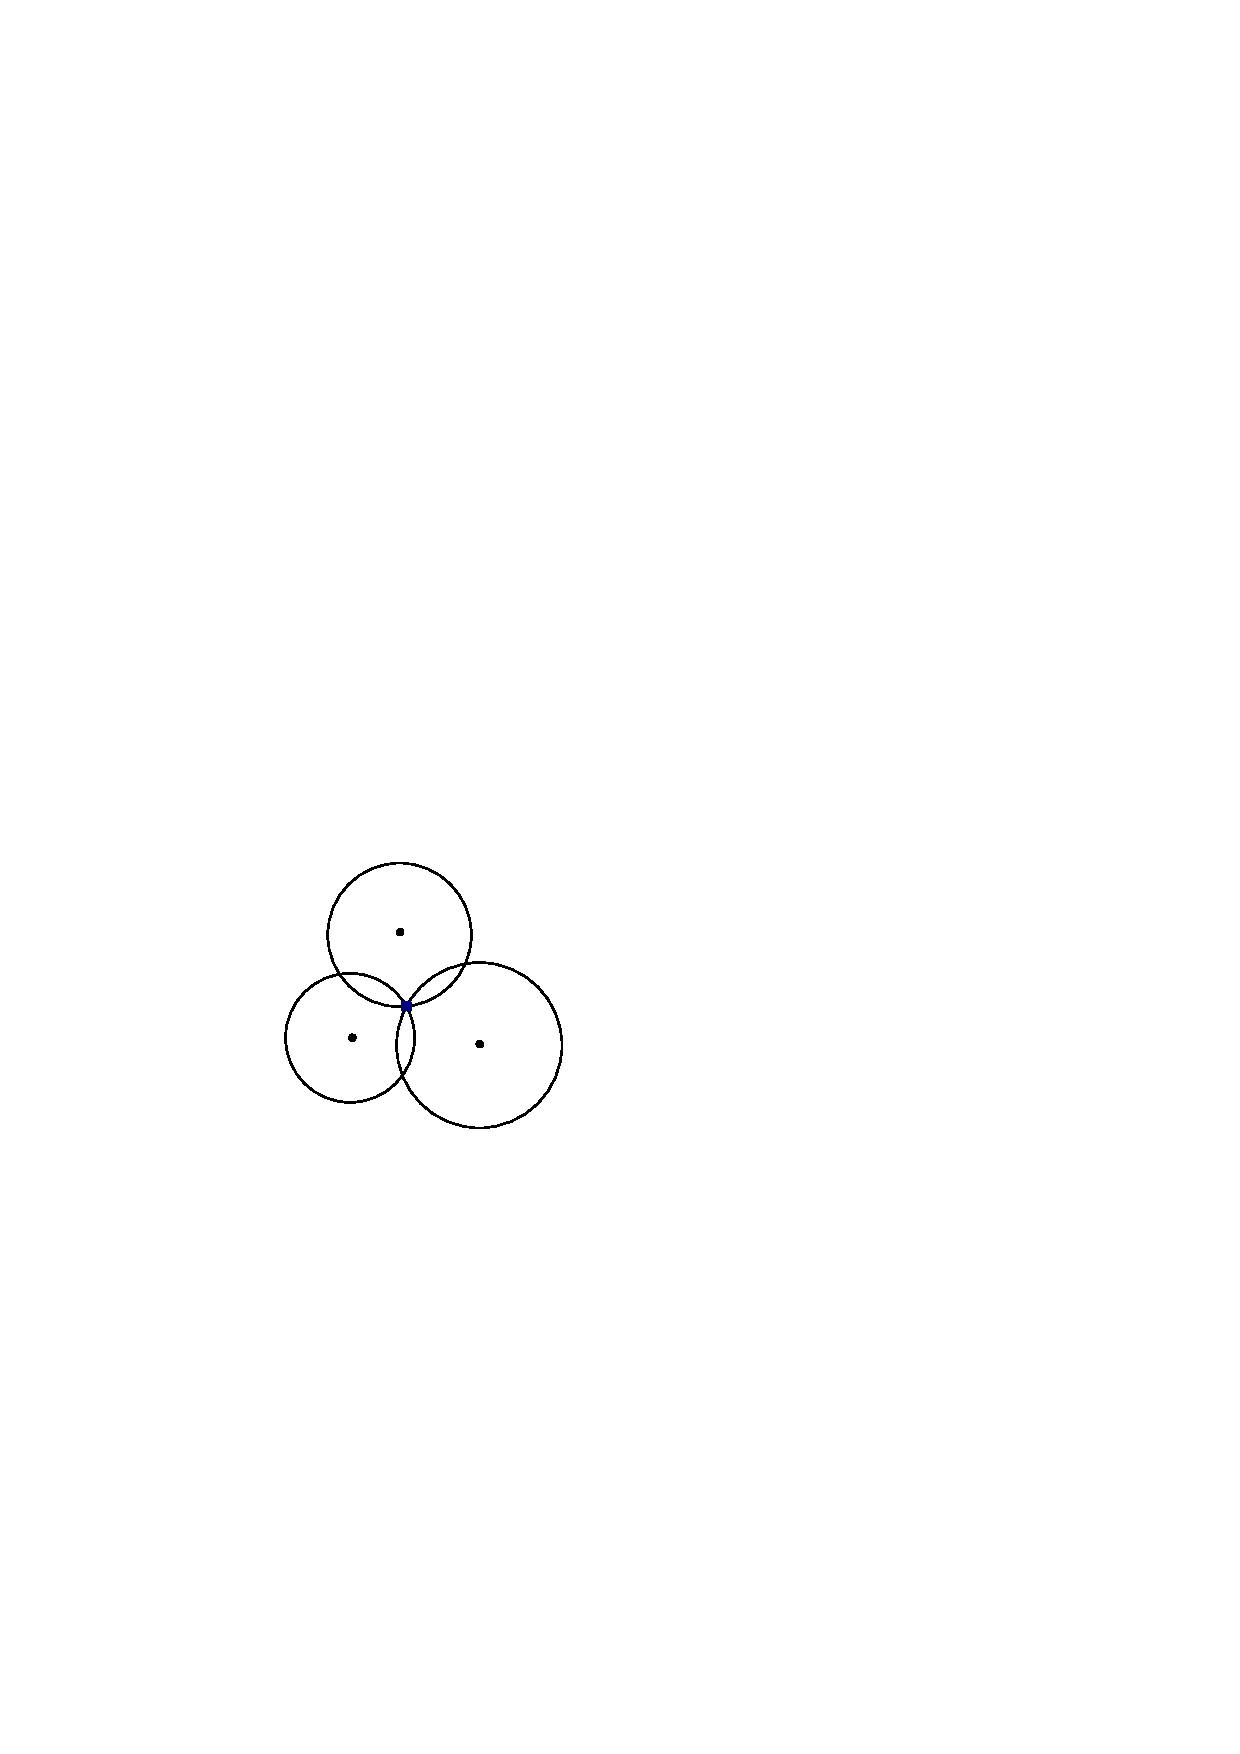
\includegraphics[width=0.19\textwidth]{images_sensor/1a.pdf} \label{fig:triletaration-a}} \hspace{5pt}
    \subfigure[three sensors]{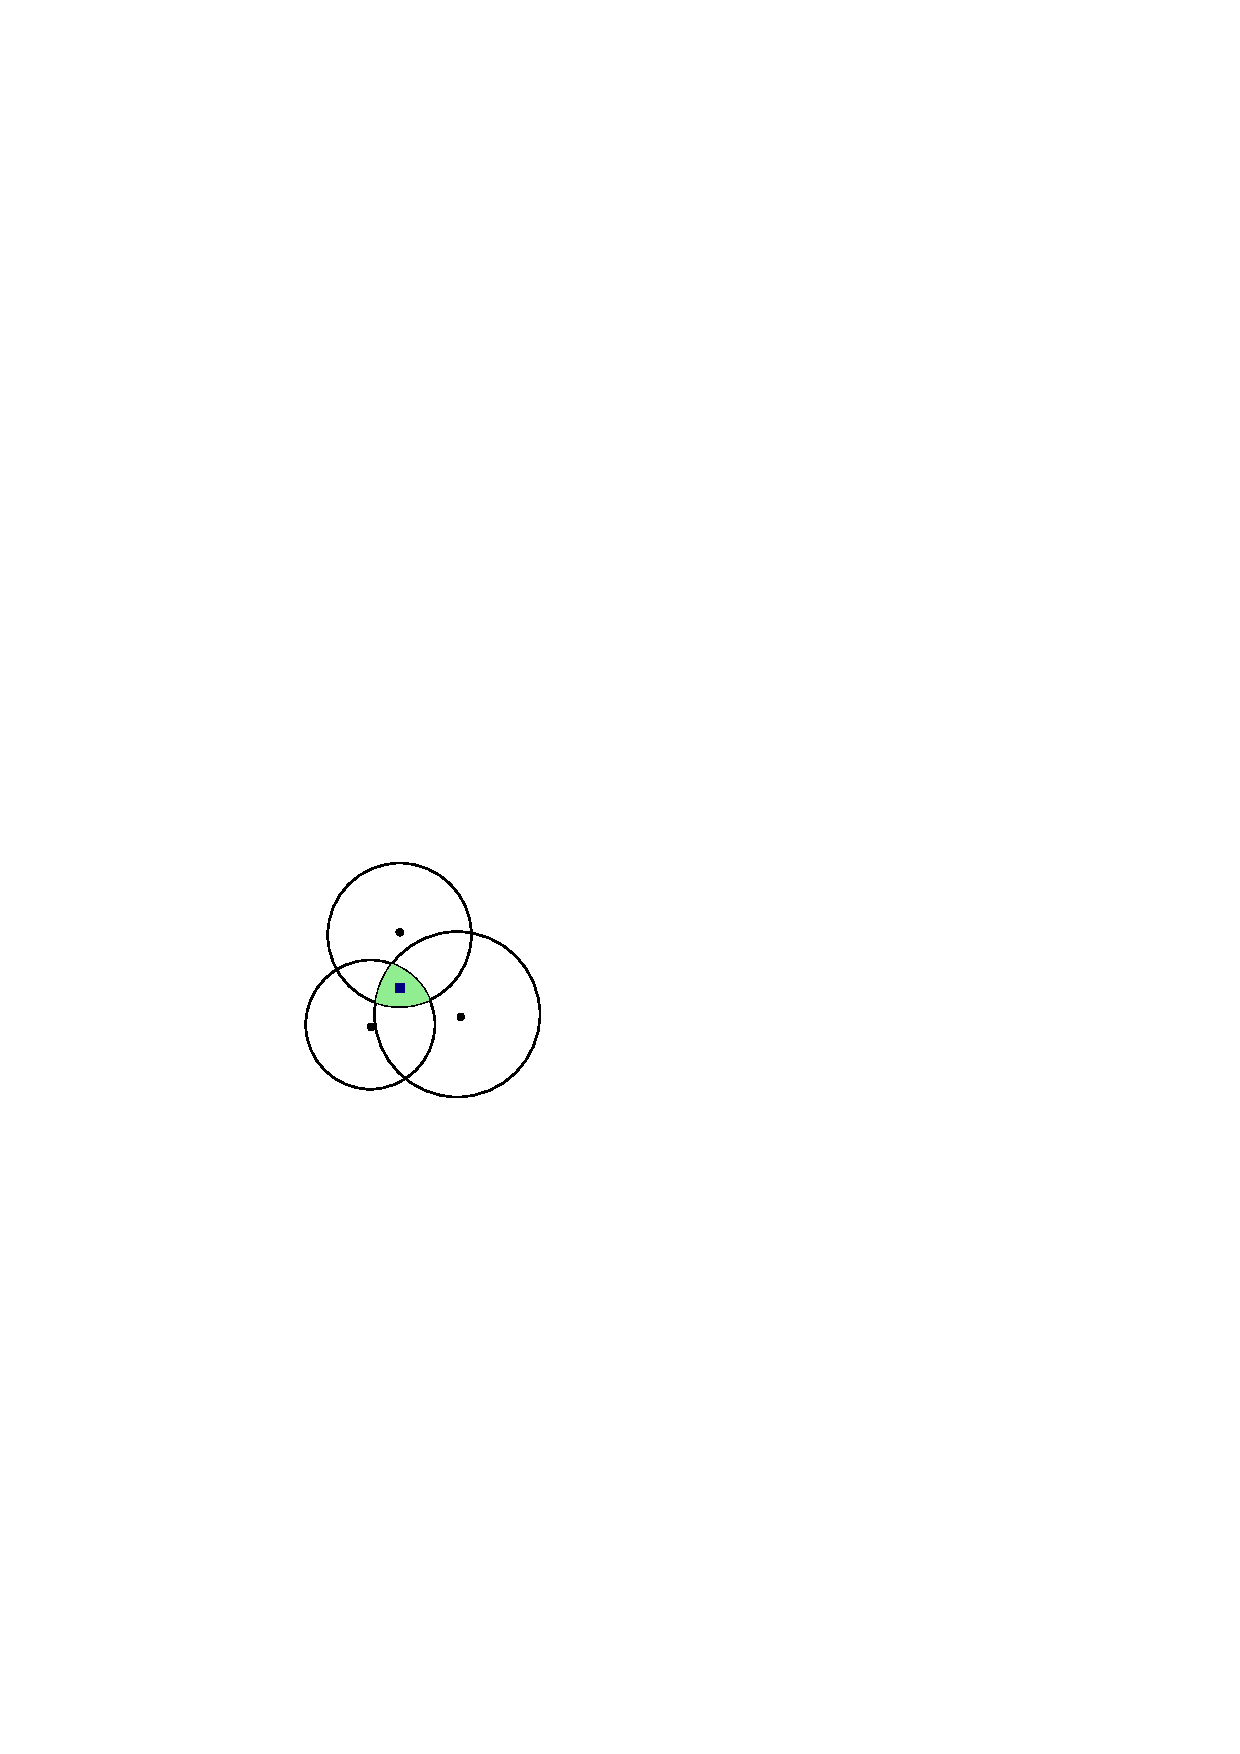
\includegraphics[width=0.19\textwidth]{images_sensor/1b.pdf} \label{fig:triletaration-b}} \hspace{5pt}
    \subfigure[multiple sensors]{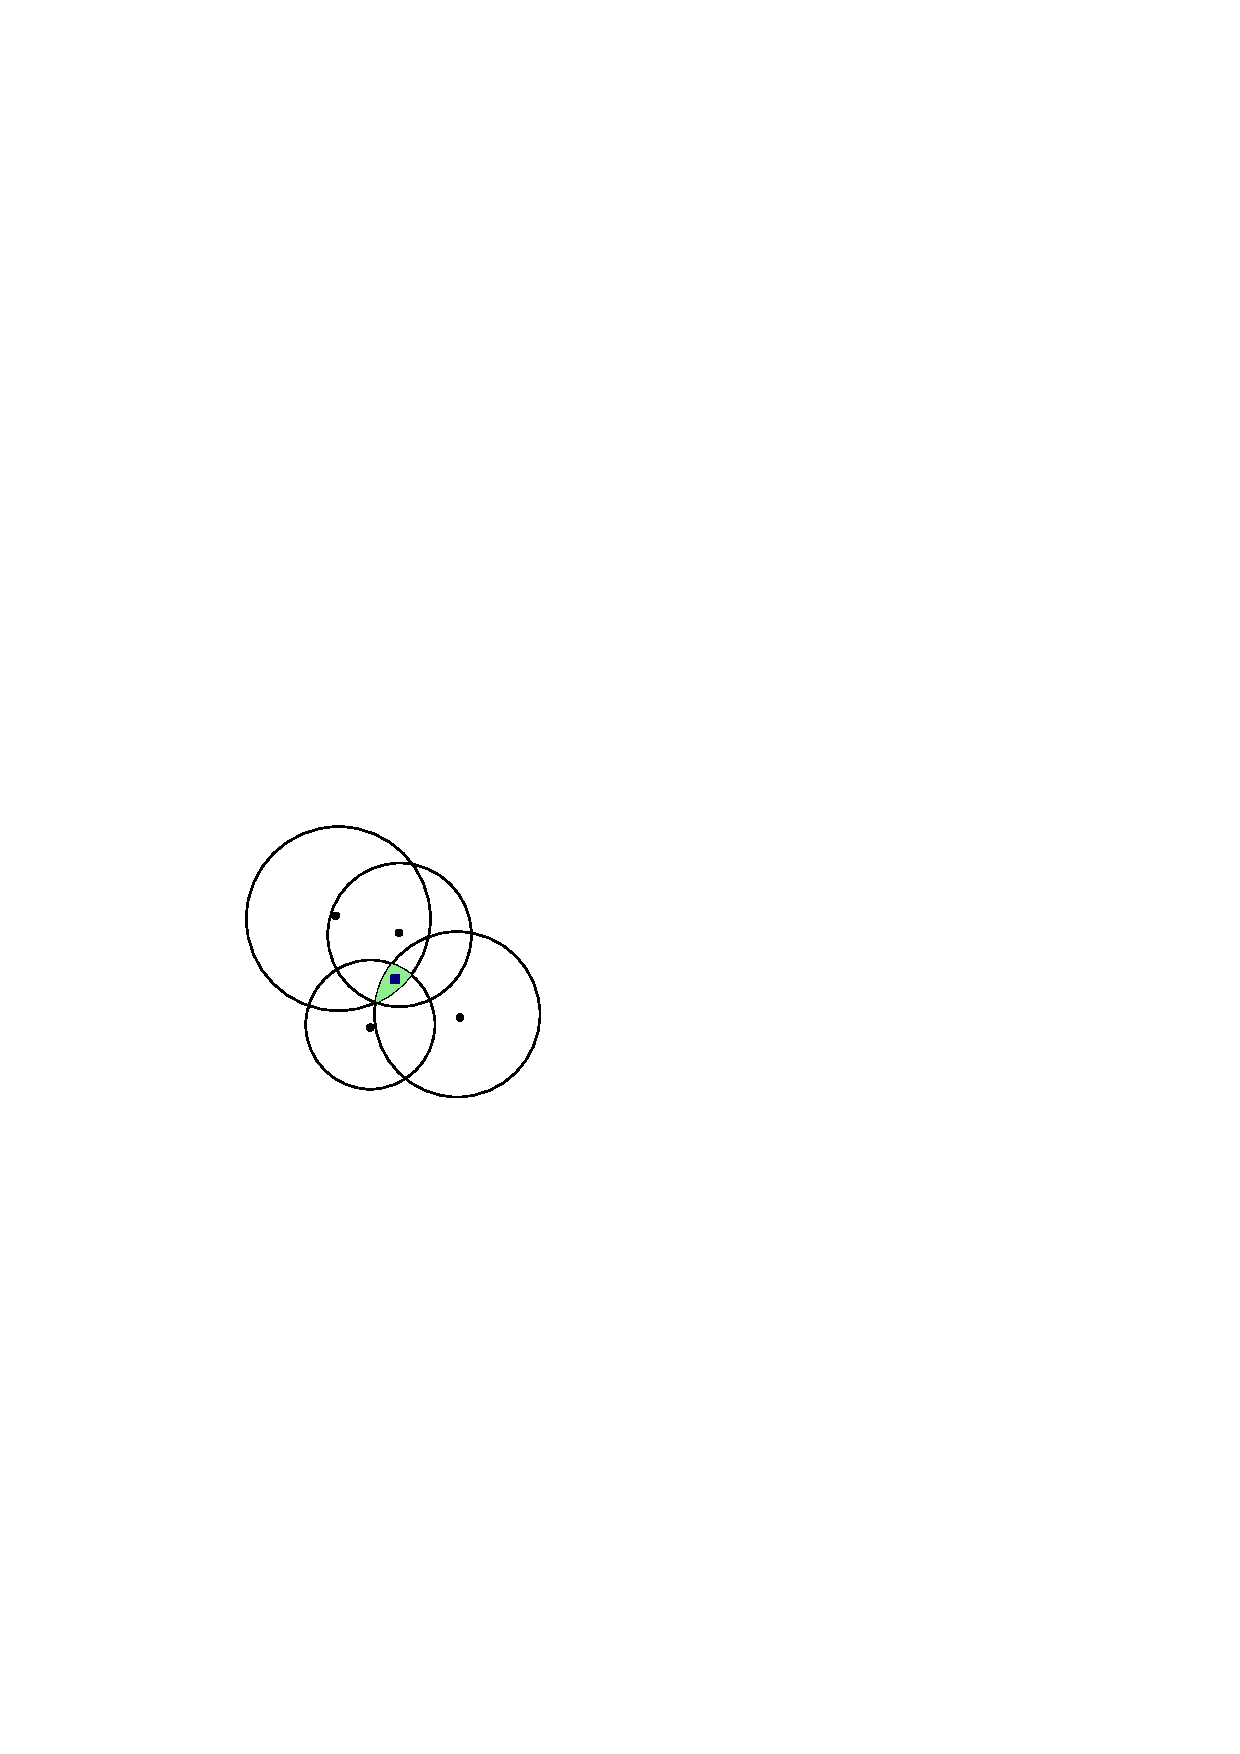
\includegraphics[width=0.19\textwidth]{images_sensor/1c.pdf} \label{fig:triletaration-c}} \hspace{5pt}
    \subfigure[disruption scenario]{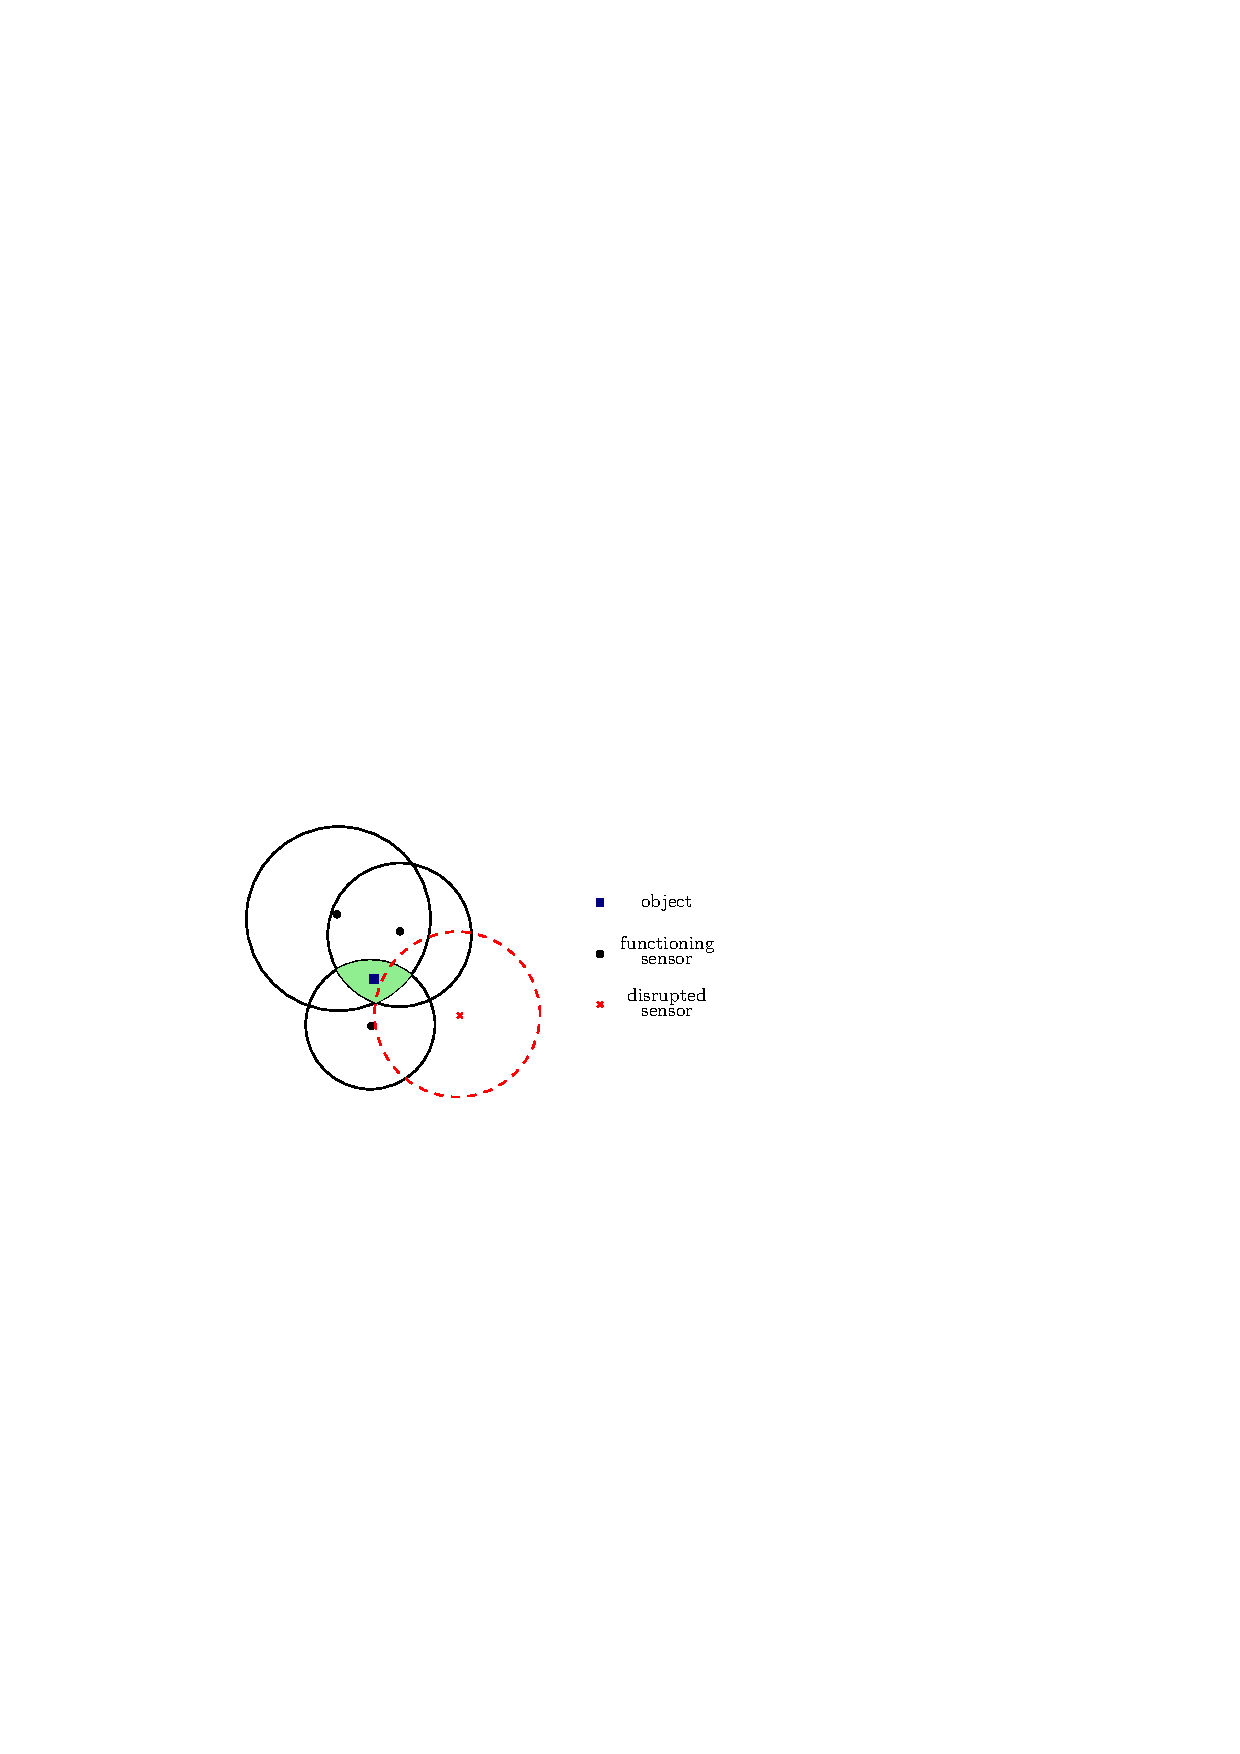
\includegraphics[width=0.32\textwidth]{images_sensor/1d.pdf} \label{fig:triletaration-d}}
  \caption{Position error illustration in trilateration.}
  \label{fig:illustration-trilateration}
\end{figure}

The remainder of this chapter is organized as follows. Section \ref{sensor:formulation} introduces the methodology we develop for the reliable sensor deployment problem, including the effectiveness measurements and the model formulation. Section \ref{sensor:algorithm} presents the solution algorithm. Section \ref{sensor:numerical} demonstrates the applicability of the model and solution algorithm on a series of examples.



\section{Model Formulation}\label{sensor:formulation}

This sensor location problem (SLP) can now be formulated as the following mixed-integer non-linear program:
\begin{subequations}
  \begin{align}
    (\text{SLP}) \quad \min_{\mathbf{X,Y,Z,P}} & \quad \sum_{j\in J} f_{j}X_{j} - \alpha\sum_{i\in I}\sum_{k\in K}\sum_{r=1}^{|\mathcal{J}|} v_{i}e_{ik}P_{ikr}Y_{ikr} \label{eqn:opt-a} \\
   \text{s.t.} & \quad \sum_{r=1}^{|\mathcal{J}|} Z_{ijr}\le X_{j}, ~\forall j\in J, i\in I, \label{eqn:opt-b} \\
   & \quad \sum_{r=1}^{|\mathcal{J}|} Z_{ijr}\le 1, ~\forall j\in J, i\in I, \label{eqn:opt-c}
  \end{align}
\end{subequations}


\begin{prop} 
  \label{prop:1}
    The assignment probability $P_{ikr}$ can be calculated recursively by \eqref{eqn:opt-b}.
\end{prop} 

\begin{proof}
  We substitute $P_{ikr-1}$ in the right hand side of \eqref{eqn:opt-c},
  \begin{align}
     P_{ikr} &= \frac{\prod_{j\in J}\left(1-p_{j}\right)^{a_{kj}}}{\prod_{j\in J}p_{j}^{a_{kj}}}\prod_{s\le r}\left[ \sum_{j\in \mathcal{J}} Z_{ijs}\left(p_{j}\right)^{1_{[j\in J]}} \right]. \label{eqn:2}
  \end{align}
  This completes the proof.
\end{proof}

\section{Solution Algorithm}\label{sensor:algorithm}
\subsection{Lagrangian Relaxation}\label{sensor:lagrangian}
In (LSLP), the sensor location variables $\mathbf{X}$ are correlated with the sensor level assignment variables $\mathbf{Z}$ by constraints \eqref{eqn:opt-b}.
\begin{subequations}
  \begin{align}
    (\text{RSLP}) \quad \min_{\mathbf{X,Y,Z,P}} & \quad \sum_{j\in J} (f_{j}-\sum_{i\in I}\mu_{ij})X_{j} \label{eqn:5-a} \\
    \text{s.t.} & \quad \eqref{eqn:opt-b} - \eqref{eqn:opt-c}. \nonumber
  \end{align}
\end{subequations}


In this way, a very large portion of the district options is eliminated from the initial set. The pseudo-code for filtering the district options is summarized as Algorithm \ref{alg:districtgenerate}.

\begin{algorithm}
  \caption{Generate the set of feasible district options}
  \label{alg:districtgenerate}
  \vskip 0.5em
  \Algorithm{DistrictGeneration}()
  \begin{algorithmic}[1]
    \FOR{$i\in \mathcal{I}$}
      \STATE{sourceHeap$ \leftarrow$ createHeap($i$), stack$ \leftarrow \emptyset$, districts$ \leftarrow \emptyset$}
      \STATE{stack.push(DFSNode($i$, sourceHeap, districts))}
      \WHILE{stack is not empty}
        \STATE{node $\leftarrow$ stack.pop()}
        \IF{ $W_{\text{weight}}\cdot$ node.demand $\cdot(1-q) + W_{\text{compact}}\cdot$ node.compact $\le \overline{W}$}
          \IF{node.hash is in districts.hashList}
            \STATE{districts.setList.add(node.set), district.hashList.add(node.hash)}
          \ENDIF
        \ENDIF
      \ENDWHILE
      \STATE{remove $i$ from $\mathcal{G}$}
    \ENDFOR
  \end{algorithmic}
  \vskip 0.5em
  \hrule
  \vskip 0.5em
  \Algorithm{createHeap}($i$, visitedNodes)
  \begin{algorithmic}[1]
    \STATE{newHeap $\leftarrow \emptyset$}
    \FOR{$n\in \mathcal{E}(i)$}
      \IF{$n$ is not in visitedNodes}
        \STATE{newHeap.insert($n$)}
      \ENDIF
    \ENDFOR
    \RETURN{ newHeap}
  \end{algorithmic}
\end{algorithm}


\section{Numerical Examples}\label{sensor:numerical}

\subsection{Hypothetical Grid Networks} \label{sensor:hypothetical}

A 2$\times$3 rectangle grid network and six $n\times n$ square grid networks for $n\in\{3,4,5,6,7,8\}$ are generated to represent various hypothetical study regions. 

\begin{table}[htbp]
  \centering
  \footnotesize
  \caption{Algorithm performance comparison for the 7 hypothetical cases.}
    \begin{tabular}{cccccccc}
    \toprule
     & Sensor  & Neighborhood  & No. of   & Final  & Final  & Final     & CPU      \\
     & network & network       & sensors  & UB     & LB     & gap (\%)  & time (s) \\
    \midrule
    \multirow{5}[2]{*}{CPLEX} 
          & $2\times3$  & $1\times2$  & 2   & -1.31    & -1.30    & 0     & 1.6   \\
          & $3\times3$  & $2\times2$  & 4   & -14.01   & fail     & 100   & 3600  \\
          & $4\times4$  & $3\times3$  & -   & -        & -        & fail  & 3600  \\
          & $\cdots$    & $\cdots$    & -   & -        & -        & fail  & 3600  \\
          & $8\times8$  & $7\times7$  & -   & -        & -        & fail  & 3600  \\
    \midrule
    \multirow{7}[2]{*}{LR+B\&B}
          & $2\times3$  & $1\times2$  & 2   & -1.31    & -1.31    & 0     & 0.1   \\
          & $3\times3$  & $2\times2$  & 4   & -24.28   & -24.28   & 0     & 0.1   \\
          & $4\times4$  & $3\times3$  & 5   & -77.38   & -77.38   & 0     & 0.4   \\
          & $5\times5$  & $4\times4$  & 8   & -150.78  & -150.78  & 0     & 0.8   \\
          & $6\times6$  & $5\times5$  & 14  & -243.48  & -243.48  & 0     & 38    \\
          & $7\times7$  & $6\times6$  & 21  & -360.99  & -360.99  & 0     & 181   \\
          & $8\times8$  & $7\times7$  & 29  & -489.07  & -500.41  & 2.32  & 3600  \\
    \bottomrule
    \end{tabular}%
  \label{tab:sensor-casestudy-stat}%
\end{table}%

\cleardoublepage


\part{Railroad Planning and Optimization}\label{part:railroad}
% !TEX root = ../ResearchBook.tex


\chapter{Integrated Planning for Multiple Types of Locomotive Work Facilities under Location, Routing, and Inventory Considerations}\label{chap:locomotive}
\chaptermark{Planning of Locomotive Facilities} % short chapter name



\section{Problem Description}\label{sec:locomotive:problem}

The assignment of repair, service, and fueling demands to various suitable facilities is determined holistically, and is represented by the solid and dashed arrows in Figure \ref{fig:locomotive:problem}.
\begin{figure}[!ht]
  \centering
    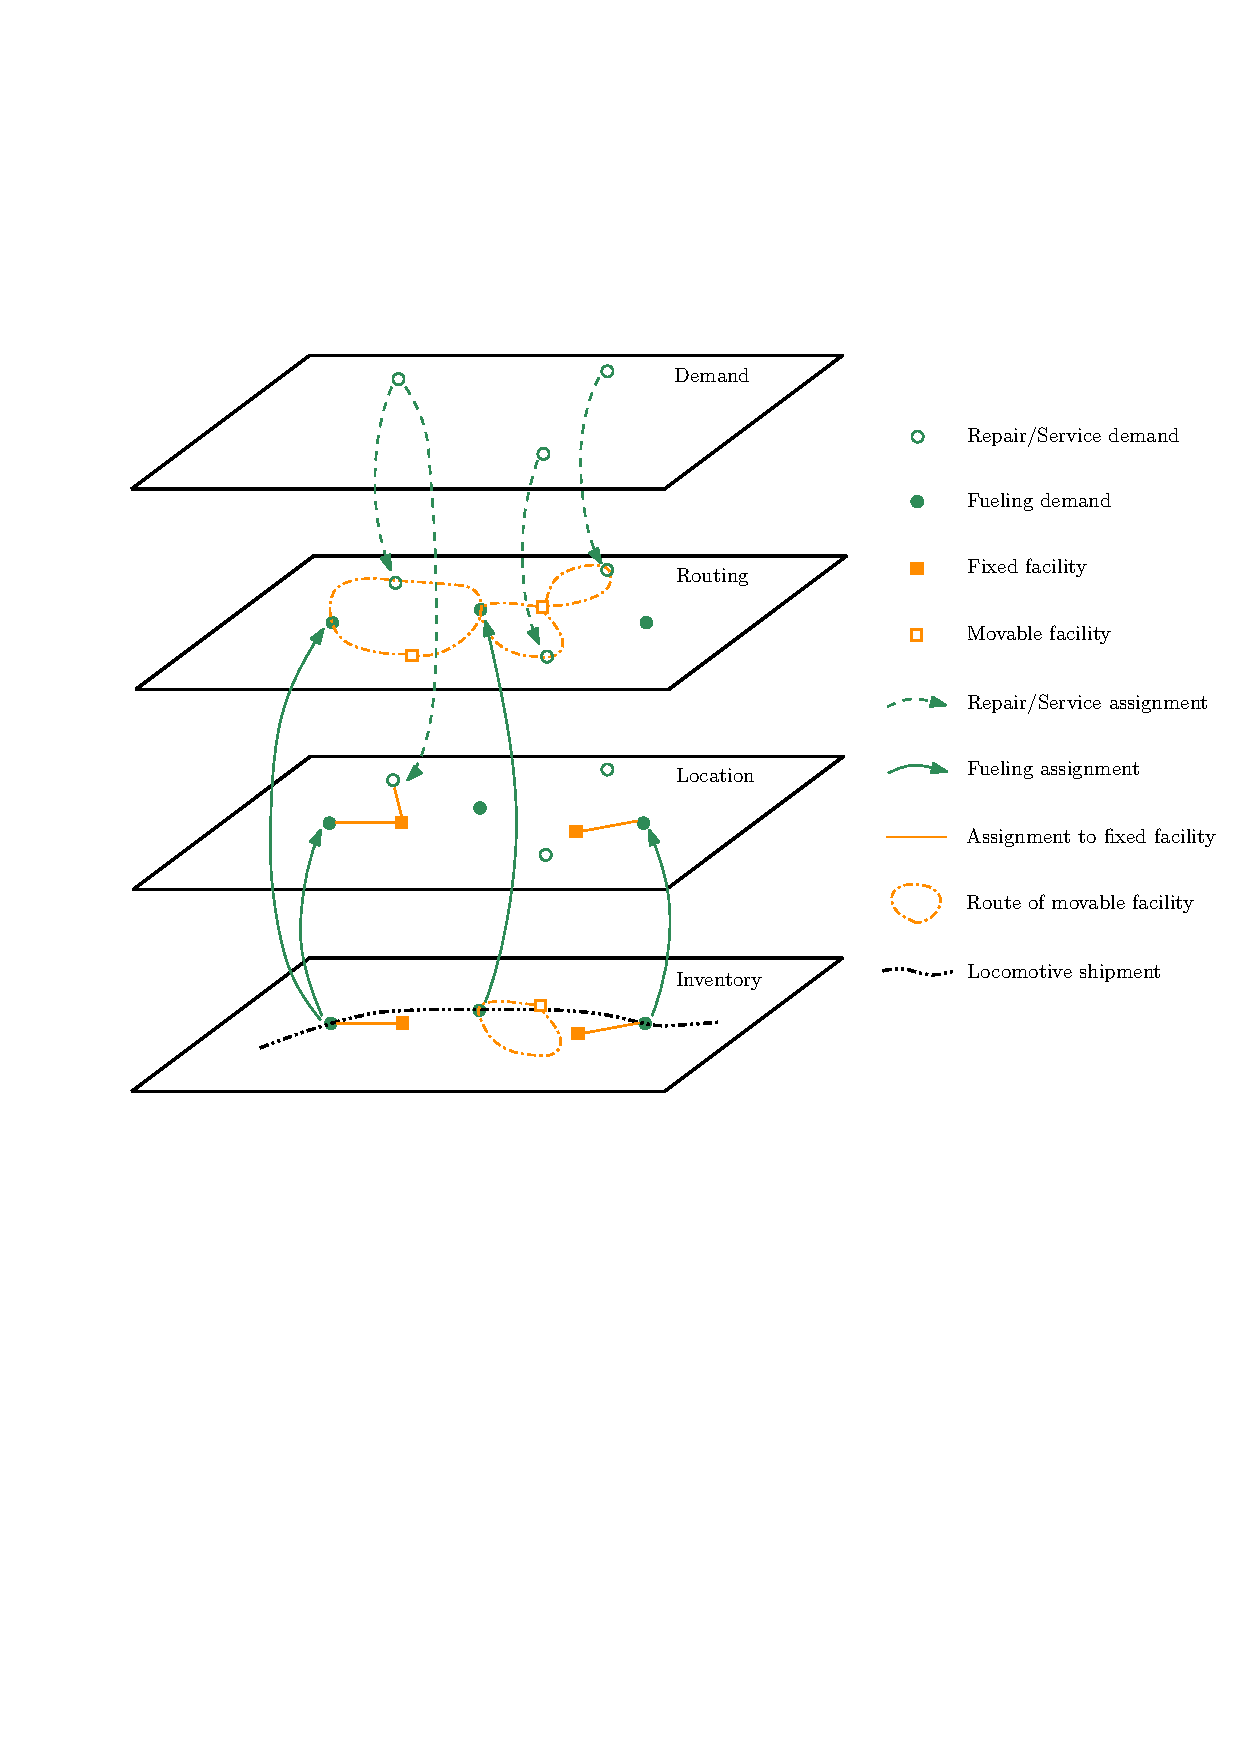
\includegraphics[width=0.75\textwidth]{images_locomotive/Figure1.pdf}
  \caption{The planning problems consist of multiple layers of decisions.} 
  \label{fig:locomotive:problem}
\end{figure}



\section{Model Formulation}\label{sec:locomotive:formulation}

In this section, we present the model formulation of solving the integrated locomotive facility planning problem, with explaination of the network transformation methods in mathematical details.


\subsection{Notation}\label{sec:locomotive:notation}
We first describe the notation used in the model formulation.

\subsubsection{Sets}
\begin{tabular}{ll}  % first type of notation list
    $\mathcal{F}$            & set of fixed facility types.  \\
    $\mathcal{M}$            & set of movable facility types.  \\
    $\mathcal{S}$            & set of work types, excluding fueling.  \\
\end{tabular}

\subsubsection{Parameters} 
\begin{notation}   % second type of notation list
  \item[$F_{n}^{\alpha}$] Annual fixed cost of operating a facility of type $\alpha$ at candidate location $n$.
  \item[$C_{n}^{\alpha}$] Cost of unit capacity at a facility of type $\alpha$ at yard $n$.
  \item[$Q_{n}^{\alpha,\max}$] Maximum (minimum) allowable capacity of facility type $\alpha$ at yard $n$.
\end{notation}

\subsection{Location-Inventory Problem Formulation}\label{sec:locomotive:location-inventory}
Below, we present the formulation for the location-inventory problem.

\subsubsection{Objective}
\begin{align*}
   \text{Minimize} ~ & \sum_{\alpha \in \mathcal{F}\cup\mathcal{M}} \sum_{n\in \mathcal{N}_{\alpha}} x_{n}^{\alpha} F_{n}^{\alpha} + \sum_{\alpha \in \mathcal{F}}\sum_{n\in \mathcal{N}_{\alpha}} q_{n}^{\alpha} C_{n}^{\alpha} + \sum_{l\in \mathcal{M}}\sum_{n\in \mathcal{N}_{l}}\left( h_{n}^{l}\cdot F_{l} + t_{n}^{l}\cdot V_{l} \right) \\
  & + \sum_{r\in\mathcal{R}}\sum_{s\in \mathcal{S}_{r}}E_{r}\left[ h_{r}^{s}\sum_{n\in \mathcal{N}}\left(G_{r,s}^{n}\cdot C_n\right) + p_{r}^s\sum_{n\in \mathcal{N}}\left(G_{r,s}^n\cdot C_{n,0}\right) \right]
\end{align*}



\section{Solution Approach}\label{sec:locomotive:algorithm}

\begin{figure}[!htbp]
\centering
    \subfigure[Transformation for train network \citep{xie2014planning}]{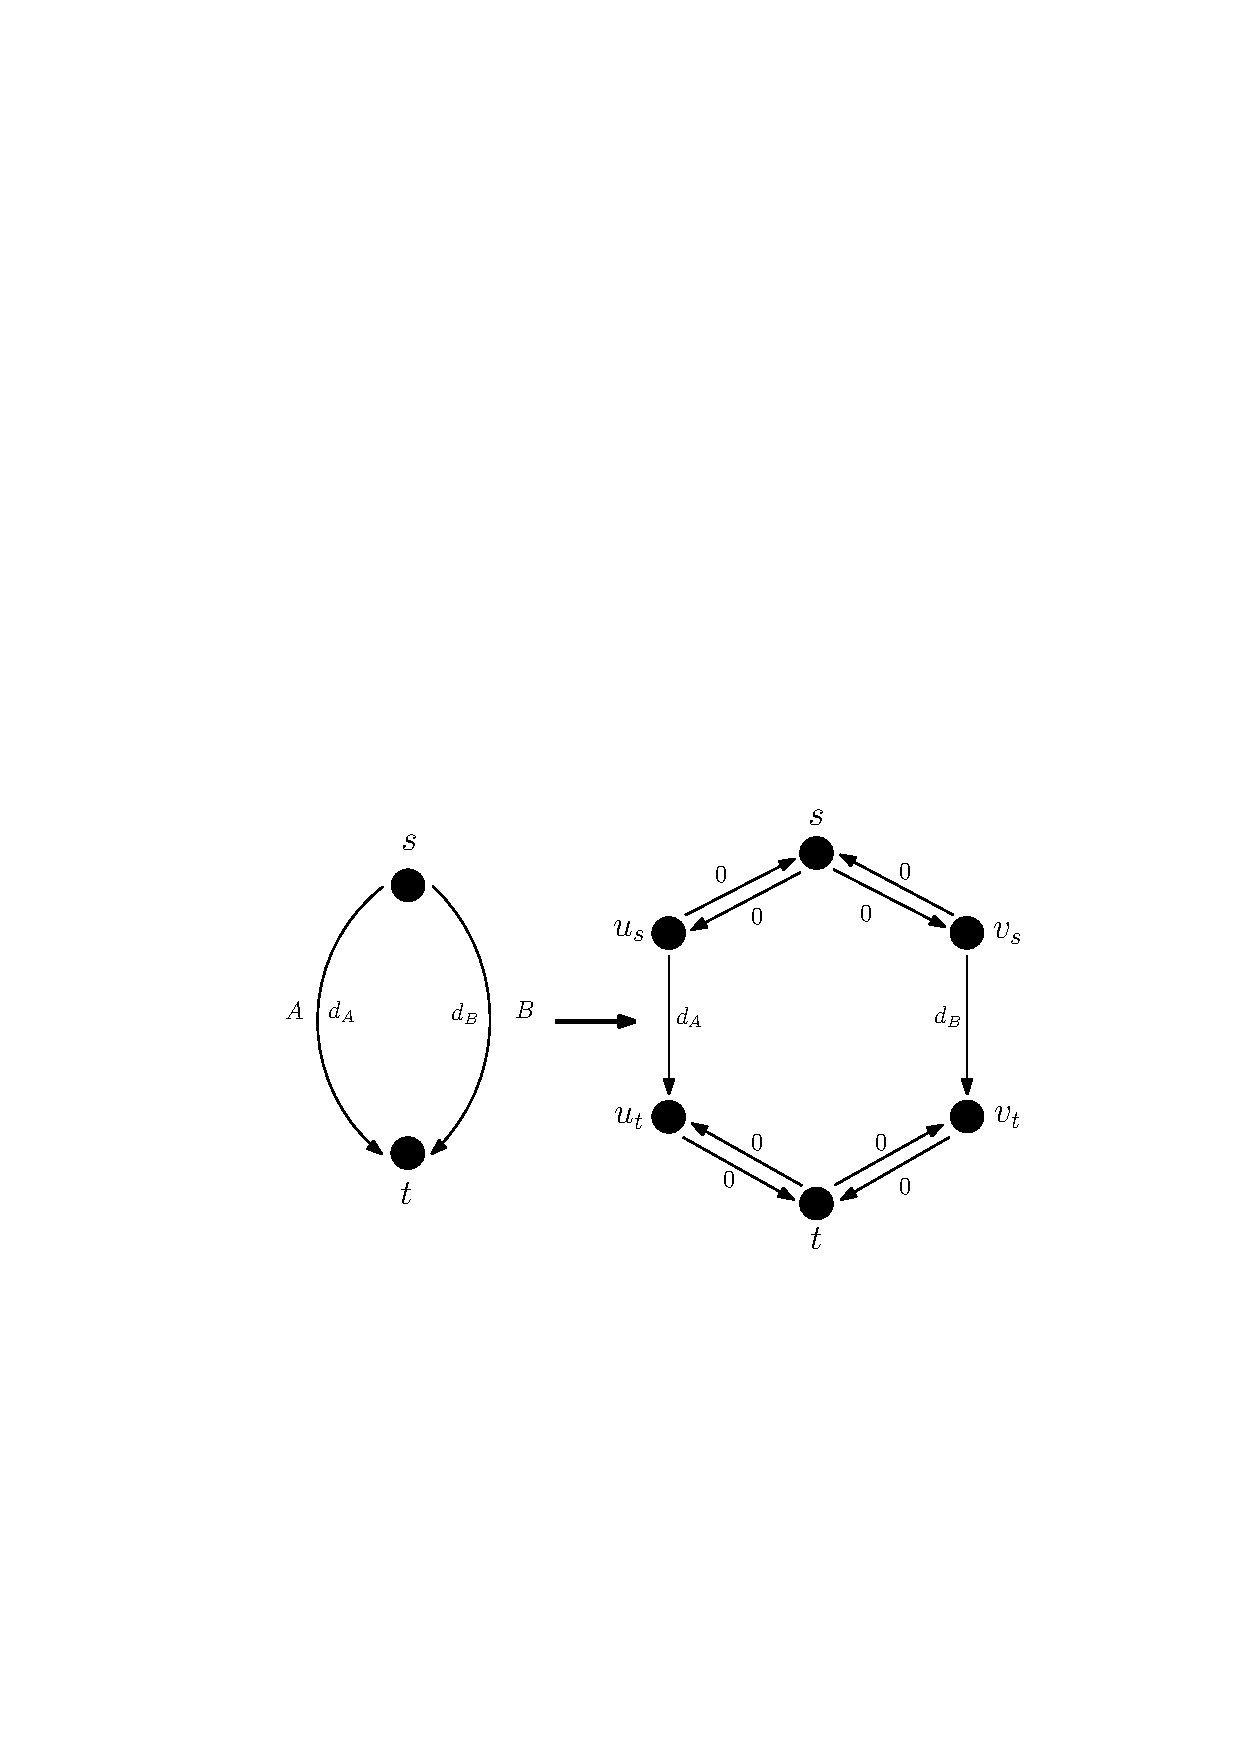
\includegraphics[width = 0.5\textwidth]{images_locomotive/Figure5a.pdf}\label{fig:Figure5a}}\hspace{15pt}
    \subfigure[Transformation for free-move network]{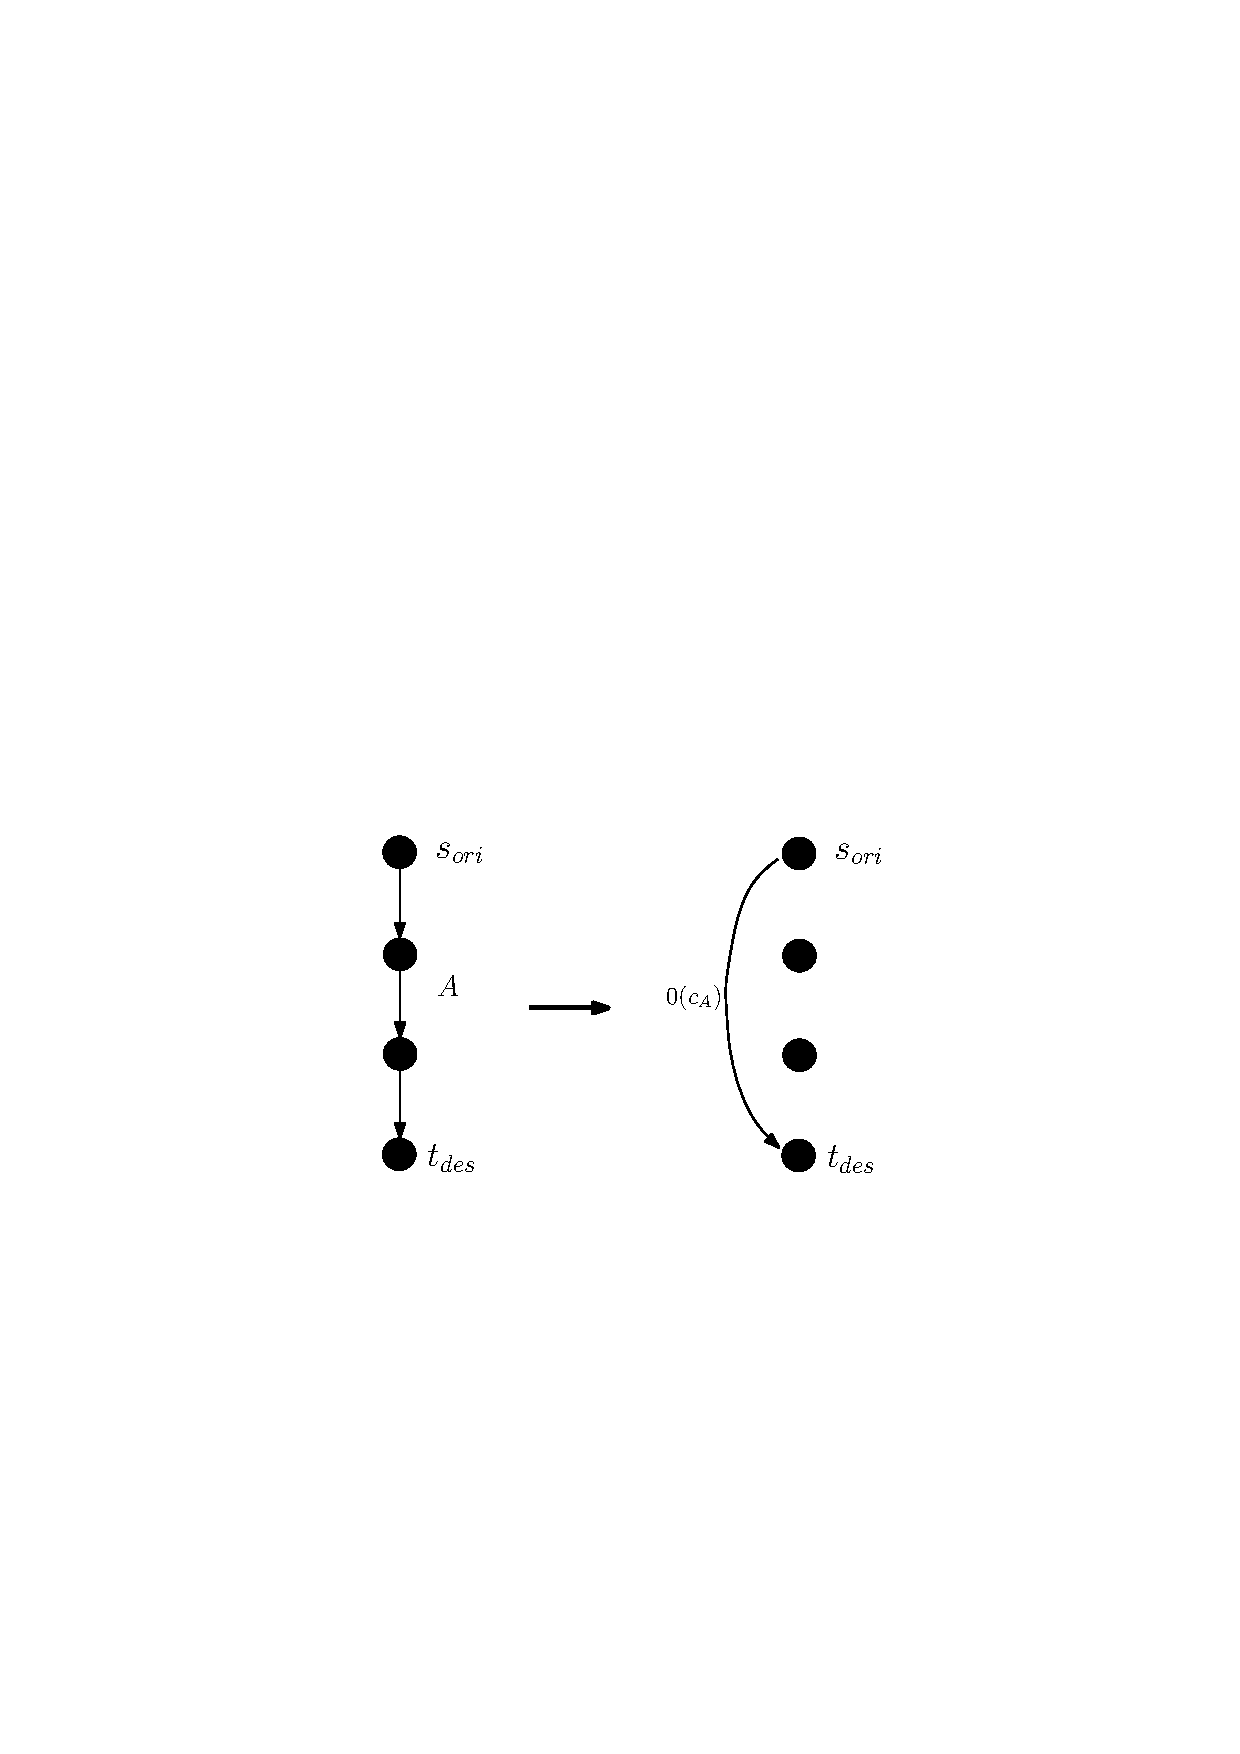
\includegraphics[width=0.4\textwidth]{images_locomotive/Figure5b.pdf}\label{fig:Figure5b}}
    \caption{The two figures illustrate how we transform train network and free-move network by adding new nodes and new edges.}
    \label{fig:Figure5}
\end{figure}


\section{Field Implementation}\label{sec:locomotive:implementation}

We implemented the presented algorithm in C\# on a computer with a three-GHz CPU and four GB of RAM.

\setcounter{table}{1}
\begin{table}[!ht]
 \centering
  \begin{tabular}{cccccccc}
    \hline
        \multirow{2}{*}{Cost} && \multirow{2}{*}{total} & \multirow{2}{*}{capacity}  & locomotive  & \multirow{2}{*}{truck} & regular  & vendor\\
        & &  &   & shipping  &   & fueling & fueling\\
    \hline
        Change ($10^6$ \$) && -72.25 & -0.68  & -109.34  & 36.02  & -7.40  & 6.75 \\
    \hline
   \end{tabular}%
  \caption{We summarize our comparison of the clean-slate scenario and base-case solutions.}%
  \label{tab:Table2}
\end{table}

\begin{table}[!ht]
  \footnotesize
  \centering
  \begin{tabular}{ccccccccc}
    \hline
        &&\multirow{2}{*}{Cost} & \multirow{2}{*}{total} & \multirow{2}{*}{capacity}  & locomotive  & \multirow{2}{*}{truck} & regular  & vendor\\
        &&  &  &   & shipping  &   & fueling & fueling\\
    \hline
        Scenario 1 &&change ($10^6$ \$) & -14.32 & 0.17  & -13.67  & -0.01  & 1.87 & -2.69 \\
    \hline
        Scenario 2 &&change ($10^6$ \$) & -44.90 & 0  & -69.06  & 4.00  & -20.73  & 40.91 \\
    \hline
   \end{tabular}%
  \caption{We summarize our comparison of the incremental scenarios and base-case solutions.}%
  \label{tab:Table3}
\end{table}






\cleardoublepage



%********************************************************************
% Backmatter
%********************************************************************
%********************************************************************
% Bibliography
%*******************************************************
% work-around to have small caps also here in the headline
% https://tex.stackexchange.com/questions/188126/wrong-header-in-bibliography-classicthesis
% Thanks to Enrico Gregorio
\defbibheading{bibintoc}[\bibname]{%
  \phantomsection
  \manualmark
  \markboth{\spacedlowsmallcaps{#1}}{\spacedlowsmallcaps{#1}}%
  \addtocontents{toc}{\protect\vspace{\beforebibskip}}%
  \addcontentsline{toc}{chapter}{\tocEntry{#1}}%
  \chapter*{#1}%
}
\printbibliography[heading=bibintoc]

% Old version, will be removed later
% work-around to have small caps also here in the headline
%\manualmark
%\markboth{\spacedlowsmallcaps{\bibname}}{\spacedlowsmallcaps{\bibname}} % work-around to have small caps also
%\phantomsection
%\refstepcounter{dummy}
%\addtocontents{toc}{\protect\vspace{\beforebibskip}} % to have the bib a bit from the rest in the toc
%\addcontentsline{toc}{chapter}{\tocEntry{\bibname}}
%\label{app:bibliography}
%\printbibliography



\end{document}
